\pdfoutput=1
%% ****** Start of file apstemplate.tex ****** %
%%
%%
%% This file is part of the APS files in the REVTeX 4 distribution.
%% Version 4.1r of REVTeX, August 2010
%%
%%
%% Copyright (c) 2001, 2009, 2010 The American Physical Society.
%%
%% See the REVTeX 4 README file for restrictions and more information.
%%
%
% This is a template for producing manuscripts for use with REVTEX 4.0
% Copy this file to another name and then work on that file.
% That way, you always have this original template file to use.
%
% Group addresses by affiliation; use superscriptaddress for long
% author lists, or if there are many overlapping affiliations.
% For Phys. Rev. appearance, change preprint to twocolumn.
% Choose pra, prb, prc, prd, pre, prl, prstab, prstper, or rmp for journal
% Add 'draft' option to mark overfull boxes with black boxes
% Add 'showpacs' option to make PACS codes appear
% Add 'showkeys' option to make keywords appear
\documentclass[aps,prd,twocolumn,superscriptaddress,preprintnumbers,floatfix,nofootinbib]{revtex4-2}
%\documentclass[aps,prl,preprint,superscriptaddress]{revtex4-1}
%\documentclass[aps,prl,reprint,groupedaddress]{revtex4-1}

\usepackage{graphicx}
\usepackage{amsmath}
%\usepackage{mdwlist}
\usepackage[caption=false]{subfig}
\usepackage{siunitx}
\usepackage{placeins}
\usepackage{color}
\usepackage{standalone}
\usepackage{dcolumn}
\usepackage{tensor}
\usepackage{bm}
%\usepackage{MnSymbol}
\usepackage{microtype}
\usepackage{etoolbox}
\usepackage{amssymb}
\usepackage{mathrsfs}
\usepackage{accents}
\usepackage[normalem]{ulem}
\usepackage[dvipsnames]{xcolor}
\usepackage[colorlinks,urlcolor=NavyBlue,citecolor=NavyBlue,linkcolor=NavyBlue,pdfusetitle]{hyperref}
\usepackage[all]{hypcap}
\usepackage[inline]{enumitem}
\usepackage[utf8]{inputenc}
\usepackage{csquotes}
\usepackage{array}
\usepackage{booktabs}

\newcommand{\ts}{\textsuperscript}

\newcommand{\beq}{\begin{equation}}
\newcommand{\eeq}{\end{equation}}

\newcommand{\nn}{\nonumber}

\newcommand*{\eq}[1]{Eq.~\eqref{eq:#1}}
\newcommand*{\fig}[1]{Fig.~\ref{fig:#1}}
\newcommand*{\sect}[1]{Sec.~\ref{sec:#1}}

\newcommand{\boldmu}{\boldsymbol{\mu}}
\newcommand{\boldn}{\mathbf{n}}
\newcommand{\boldd}{\mathbf{d}}
\newcommand{\bolds}{\mathbf{s}}
\newcommand{\boldSigma}{\boldsymbol{\Sigma}}

\newcommand{\area}{\mathcal{A}}

%% Try to control orphans, widows, and extra whitespace
%\widowpenalty=10000
%\clubpenalty=10000
%\raggedbottom
\interfootnotelinepenalty=3000

%% Enable/disable comments
\newtoggle{commentsoff}
\togglefalse{commentsoff}
%\toggletrue{commentsoff}

% Check for command-line option to turn comments off
% https://tex.stackexchange.com/questions/1492/passing-parameters-to-a-document
\ifdefined\nocomments
    \toggletrue{commentsoff}
\fi

\iftoggle{commentsoff}{
  \newcommand*{\mi}[1]{}
  \newcommand*{\mg}[1]{}
  \newcommand*{\wf}[1]{}
  \newcommand*{\comment}[1]{}
  \newcommand*{\suggest}[3]{#2}
  \newcommand*{\todo}[1]{}
  \newcommand*{\warn}[1]{}
  \newcommand*{\red}[1]{#1}
  \newcommand*{\blue}[1]{#1}
  \newcommand{\cn}{}
  \newcommand*{\commentmark}[1]{}
}{
  \newcommand*{\mi}[1]{{\color{magenta} [{\bf MAX}: #1]}}
  \newcommand*{\wf}[1]{\textcolor{green}{\textbf{WILL}: #1}}
  \newcommand*{\suggest}[3]{\textcolor{Purple}{\textbf{#3} \sout{#1} #2}}
  \newcommand*{\comment}[1]{{\color{blue} [{\bf NOTE}: #1]}}
  \newcommand*{\warn}[1]{{\color{red} [{\bf WARNING}: #1]}}
  \newcommand*{\todo}[1]{{\color{red} [{\bf TODO}: #1]}}
  \newcommand*{\red}[1]{{\color{purple} #1}}
  \newcommand*{\blue}[1]{{\color{blue} #1}}
  \newcommand{\cn}{\blue{\bf [cn]}}
}

\graphicspath{{./fig/}}

\newcommand{\dcc}{LIGO-PXXXXXXX}

% NOTATION MACROS
\newcommand{\infd}{\mathrm{d}}
\newcommand{\white}{\bar}

\newcommand{\snropt}{\mathrm{SNR}}
\newcommand{\snrmf}{\mathrm{SNR}_{\rm mf}}
\newcommand{\cov}{C}
\newcommand{\acf}{\rho}
\newcommand{\nmode}{D}

\begin{document}

% Use the \preprint command to place your local institutional report
% number in the upper righthand corner of the title page in preprint mode.
% Multiple \preprint commands are allowed.
% Use the 'preprintnumbers' class option to override journal defaults
% to display numbers if necessary
% \preprint{\dcc}

%Title of paper
\title{Parametrizing gravitational-wave polarizations}

\author{Maximiliano Isi}
\email[]{maxisi@mit.edu}
\thanks{NHFP Einstein fellow}
%\homepage[]{Your web page}
%\thanks{}
%\altaffiliation{}
\affiliation{
LIGO Laboratory, Massachusetts Institute of Technology, Cambridge, Massachusetts 02139, USA
}%
%\affiliation{Center for Computational Astrophysics, Flatiron Institute, 162 5th Ave, New York, NY 10010}

% Because hyperref only gets the *last* author, we need to be explicit.
\hypersetup{pdfauthor={Isi}}

\date{\today}

\begin{abstract}
Amazing!
\end{abstract}

\maketitle

% \tableofcontents

\section{Introduction}
\label{sec:intro}

It is useful to parametrize gravitational-wave (GW) polarizations in different ways.
Here I outline some useful alternatives and show how they are related.
It is important to understand the priors implied by the choice of parametrization through the corresponding Jacobians.

\section{General relativity}

\subsection{Polarizations}
\label{sec:pol}

In GR, there exist two propagating gravitational degrees of freedom, corresponding to two independent GW polarizations (e.g., \cite{Thorne:1987af}).
Their local effect can be encoded in a driving matrix $h_{ij}$ representing the transverse-traceless part of the metric perturbation.
In a frame with $z$-axis along the direction of propagation, we can write this as
\beq \label{eq:hij}
(h_{ij}) = \begin{pmatrix}
h_+ & h_\times  & 0 \\
h_\times  & - h_+ & 0  \\
0 & 0 & 0
\end{pmatrix} ,
\eeq
where the plus ($+$) and cross ($\times$) polarization functions, $h_{+/\times}$, are implicit functions of the retarded time, $t - R/c$, to be specified by the source dynamics and the distance $R$ to the source.
It can be useful to rewrite \eq{hij} as $h_{ij} = h_+ e^+_{ij} + h_\times e^\times_{ij}$, making use of the polarization tensors
\beq
e^+_{ij} \equiv \hat{x}_i \hat{x}_j - \hat{x}_i \hat{x}_j \, ,
\eeq
\beq
e^\times_{ij} \equiv \hat{x}_i \hat{y}_j + \hat{x}_i \hat{y}_j\, ,
\eeq
where $\hat{x}$ and $\hat{y}$ are orthonormal vectors that, with $\hat{z}$, form a right-handed Cartesian basis.
We will call this the \emph{wave frame}.

Equation \eqref{eq:hij} presumes a specific choice of frame orientation that defines the basis in which the $h_{ij}$ components are written.
Although \eq{hij} requires that $\hat{z}$ be parallel to the (spatial) wave vector $\vec{k}$, there is no a priori restriction on the orientation of the $x$ and $y$ axes within the plane perpendicular to $\vec{k}$.
This freedom is usually encapsulated in the choice of an arbitrary \emph{polarization angle} $\psi$, defined with respect to some convenient reference (e.g., the celestial equator \cite{LALSuite:wave}).
With some trigonometry, it is straightforward to show that a rotation by some angle $\Delta \psi$ around $z$ leaves the form of \eq{hij} unchanged after redefining
\beq \label{eq:htransf}
h_+ \rightarrow h_+' = h_+ \cos 2\Delta \psi - h_\times \sin 2\Delta\psi \, ,
\eeq
\beq
h_\times \rightarrow h_\times' = h_\times \cos 2\Delta \psi + h_+ \sin 2\Delta\psi \, .
\eeq
This reveals the fact that $h_+$ and $h_\times$ are nothing but the two components of a tensor field with spin-weight $s=2$, and the two polarizations are only defined up to an arbitrary choice of $\psi$.
In fact, we coud easily rewrite \eq{hij} in terms of the corresponding right and left handed polarizations, $h_{R/L} = h_+ \pm i h_\times$, which are invariant under $\psi$ rotations (concretely, eigenvectors of the helicity operator with eigenvalues $\pm 2$).
%Although a choice of $\psi$ is required to prescribe $h_+$ and $h_\times$ in \eq{hij}, the form of this equation is invariant under changes in $\psi$.

In the small-antenna limit, the signal induced by a passing GW on a given detector can be written as the projection
\beq \label{eq:h}
h(t) \equiv D^{ij} h_{ij} = F_+ h_+ + F_\times h_\times\, 
\eeq
with antenna patterns $F_{+/\times} \equiv D^{ij} e^{+/\times}_{ij}$ defined in terms of a detector tensor $D_{ij}$ that represents the geometry of the measurement.
For a differential-arm detector with arms pointing along unit vectors $\hat{X}$ and $\hat{Y}$, this is just $D_{ij} = (\hat{X}_i \hat{X}_j - \hat{Y}_i \hat{Y}_j)/2$.%
\footnote{These expressions are valid in the local Lorentz frame of the detector, so we can raise and lower indices with the flat metric.}
In this limit, the antenna patterns are thus purely geometric factors that encode the relative orientations of the detector and wave frames, as defined by $\{\hat{X},\, \hat{Y},\, \hat{Z}\}$ and $\{\hat{x},\, \hat{y},\, \hat{z}\}$ respectively.
Under rotations of the wave frame, they transform through an expression complementary to \eq{htransf},
\beq \label{eq:Ftransf}
F_+ \rightarrow F_+' = F_+ \cos 2\Delta \psi + F_\times \sin 2\Delta\psi \, ,
\eeq
\beq
F_\times \rightarrow F_\times' = F_\times \cos 2\Delta \psi - F_+ \sin 2\Delta\psi \, ,
\eeq
ensuring that the observable $h(t)$ in \eq{h} is independent of the arbitrary angle $\psi$.

\subsection{Elliptically polarized signals}
\label{sec:ellip}

\begin{figure}
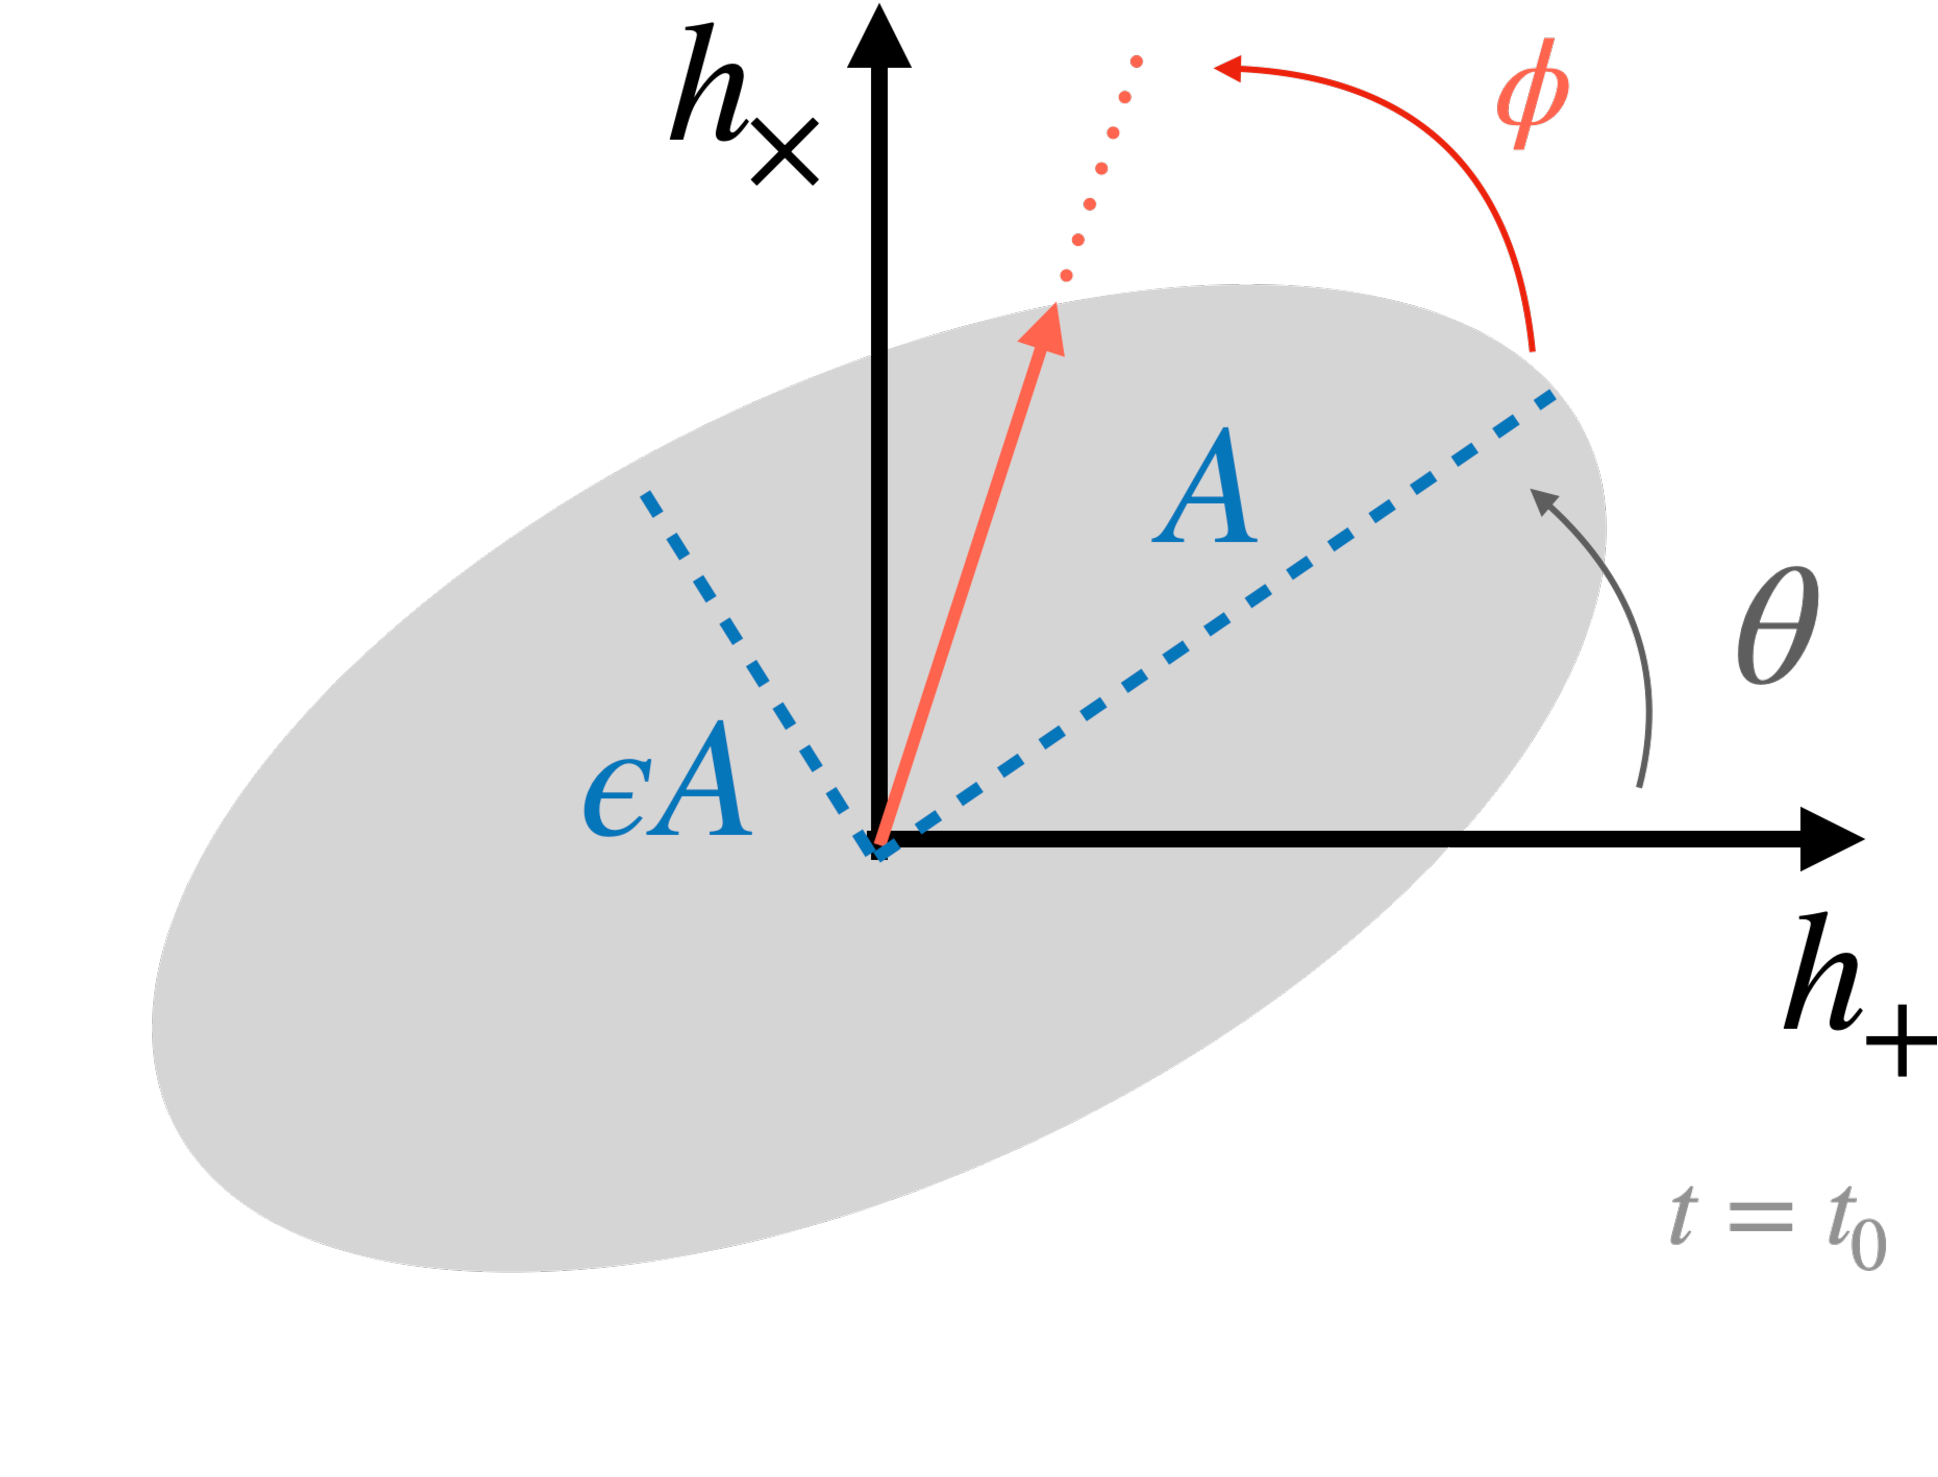
\includegraphics[width=0.6\columnwidth]{ellipse}
\caption{Polarization ellipse. At any given time, the phasor of an elliptically polarized signal lies on an ellipse with some instantaneous amplitude $A(t)$ and time-independent ellipticity $\epsilon$, with semimajor axis tilted by an angle $\theta$ with respect to the plus-polarization axis (abscissa); a second angle, $\phi \equiv \Phi(t=0)$, determines the initial location of the phasor within the ellipse. (Adapted from \cite{Isi:2021iql}.)}
\label{fig:ellipse}
\end{figure}

In full analogy to electromagnetic waves, a GW is elliptically polarized if the phasor describing the signal lies always on an ellipse in the $h_+$ vs $h_\times$ plane (Fig.~\ref{fig:ellipse}).
That means that, regardless of wave-frame orientation (equivalently, choice of $\psi$), the signal can always be put in the form
\begin{subequations} \label{eq:ellip}
\begin{equation} \label{eq:ellip_p}
h_+ = A(t) \left[\cos \Phi(t) \cos \theta - \epsilon \sin \Phi(t) \sin\theta \right] ,
\end{equation}
\begin{equation} \label{eq:ellip_c}
h_\times = A(t) \left[ \cos \Phi(t) \sin \theta + \epsilon \sin \Phi(t) \cos\theta \right] ,
\end{equation}
\end{subequations}
where $A(t)$ and $\Phi(t)$ are some amplitude and phase functions, and where the ellipticity $-1 \leq \epsilon \leq 1$ and angle $0 \leq \theta \leq \pi$ control the shape and orientation of the polarization ellipse.

% \begin{equation} \label{eq:h_ellip_lmn_plus}
% h_+ = h_c\, \cos \theta - \epsilon h_s\, \sin\theta\, ,
% \end{equation}
% \begin{equation} \label{eq:h_ellip_lmn_cross}
% h_\times = h_c\, \sin \theta + \epsilon h_s\, \cos\theta\, ,
% \end{equation}
% for cosine and sine quadratures
% \begin{equation}  \label{eq:h_ellip_lmn_sin}
% h_c \equiv A(t)\, \cos \Phi(t) \, ,
% \end{equation}
% \begin{equation} \label{eq:h_ellip_lmn_cos}
% h_s \equiv A(t)\, \sin \Phi(t) \, .
% \end{equation}

The expression for an elliptical wave simplifies if we orient $\hat{x}$ such that the plus and cross axes are aligned with the principal components of the ellipse, so that $\theta = 0$.
With such a choice of wave frame (equivalently, choice of $\psi$), the above becomes just
\begin{subequations} \label{eq:ellip_frame}
\beq
h_+ = A(t) \cos \Phi(t) \, ,
\eeq
\beq
h_\times = \epsilon A(t) \sin \Phi(t)\, ,
\eeq
\end{subequations}
for some time-independent ellipticity $-1 \leq \epsilon \leq 1$, and arbitrary amplitude and phasing functions $A(t)$ and $\Phi(t)$.
Crucially, an elliptical wave will generally not take the form of Eq.~\eqref{eq:ellip_frame} unless $\hat{x}$ is chosen appropriately; only signals with $\epsilon=\pm1$ will take  this simplified form irrespective of the wave frame orientation.

When working with a single elliptically-polarized wave, Eq.~\eqref{eq:ellip_frame} defines a privileged orientation of the wave frame, unique up to rotations by $\pi/2$ around $\hat{z}$.
If we adopt $\theta =0$ as a convention (or, equivalently, $\theta=\pi$), then we \emph{define} our wave frame to lie along the principal axes of the polarization ellipse and, thus, the polarization angle $\psi$ becomes synonymous with the polarization ellipse orientation.
However, the two angles $\theta$ and $\psi$ are conceptually distinct (in particular, $\theta$ is defined only for elliptically polarized waves, whereas $\psi$ is always defined).

% where the source sky location is parametrized by its right ascension $\alpha$ and declination $\delta$.

As for any GW, the detector output for an elliptically polarized wave will be given by \eq{h}.
In this case, however, \eq{Ftransf} implies that $\psi$ and $\theta$ are degenerate, as detailed in Appendix A of \cite{Isi:2017equ}.
Concretely, for a fixed sky location, a change from $\psi \to \psi' = \psi + \Delta\psi$ in the antenna patterns can be absorbed by a change in $\theta$ because the expression
\beq
h = F_+(\psi + \Delta \psi) h_+ + F_\times(\psi + \Delta \psi) h_\times 
\eeq
can be expanded by means of \eq{Ftransf} to read
\begin{align}
h = &\left[ F_+(\psi) \cos 2\Delta\psi + F_\times(\psi) \sin 2\Delta\psi \right] h_+\, + \\
 &\left[F_\times(\psi) \cos 2\Delta\psi - F_+(\psi)\sin 2\Delta\psi\right] h_\times \, .
\end{align}
Plugging in the expressions for an elliptical wave in \eq{ellip} and taking advantage of trigonometric identities, this can be rearranged into
\begin{widetext}
\begin{align}
h = & A(t) \left[\cos \Phi(t) \cos(\theta + 2\Delta\psi) -  \epsilon \sin \Phi(t)\sin(\theta + 2\Delta\psi) \right] F_+(\psi) +\nonumber\\
&A(t) \left[\cos \Phi(t) \sin(\theta + 2\Delta\psi) + \epsilon \sin \Phi(t) \cos(\theta + 2\Delta\psi) \right] F_\times(\psi), 
\end{align}
\end{widetext}
which is the same result we would have obtained by replacing $\theta \to \theta' = \theta + 2 \Delta\psi$ in \eq{ellip}.
This implies that, analyses that allow $\theta$ to vary freely should avoid degeneracies by fixing $\psi$ to an arbitrary a priori value, and viceversa.


% \begin{alignat}{2}
% h &= &&\left. F_+(\psi + \Delta \psi) h_+ + F_\times(\psi + \Delta \psi) h_\times\right.  \\
%   &= &&\left[ F_+(\psi) \cos 2\Delta\psi + F_\times(\psi) \sin 2\Delta\psi \right] h_+\, + \\
% & &&\left[F_\times(\psi) \cos 2\Delta\psi - F_+(\psi)\sin 2\Delta\psi\right] h_\times, 
% \end{alignat}
The (arbitrary) choice to set $\psi=0$ in the antenna pattern evaluation is legitimate because that degree of freedom is fully degenerate with the $\theta_i$ via Eq.~\eqref{eq:Ftransf}, as detailed in Appendix A of \cite{Isi:2017equ}.
Concretely, a change from $\psi = 0$ to $\psi= \Delta\psi$ can be written as
\begin{align}
h = &\left[ F_+(\psi=0) \cos 2\Delta\psi + F_\times(\psi=0) \sin 2\Delta\psi \right] h_+\, +\nonumber\\
&\left[F_\times(\psi=0) \cos 2\Delta\psi - F_+(\psi=0)\sin 2\Delta\psi\right] h_\times, 
\end{align}
suppressing the sky location dependence for simplicity.
For a given m

\begin{align}
h = & \left[h_+ \cos 2\Delta\psi - h_\times \sin 2\Delta\psi \right] F_+(\psi=0) +\nonumber\\
&\left[h_\times \cos 2\Delta\psi + h_+ \sin 2\Delta\psi\right] F_\times(\psi=0), 
\end{align}

% \begin{widetext}
% \begin{align}
% h = & \left[A(t) \left[\cos \Phi(t) \cos \theta - \epsilon \sin \Phi(t) \sin\theta \right] \cos 2\Delta\psi - A(t) \left[ \cos \Phi(t) \sin \theta + \epsilon \sin \Phi(t) \cos\theta \right]  \sin 2\Delta\psi \right] F_+(\psi=0) +\nonumber\\
% &\left[A(t) \left[ \cos \Phi(t) \sin \theta + \epsilon \sin \Phi(t) \cos\theta \right]  \cos 2\Delta\psi + A(t) \left[\cos \Phi(t) \cos \theta - \epsilon \sin \Phi(t) \sin\theta \right] \sin 2\Delta\psi\right] F_\times(\psi=0), 
% \end{align}
% \end{widetext}

\begin{widetext}
\begin{align}
h = & A(t) \left[\cos \Phi(t) \left[ \cos 2\Delta\psi\cos \theta - \sin \theta \sin 2\Delta\psi  \right] -  \epsilon  \sin \Phi(t)\left[ \cos 2\Delta\psi \sin\theta+ \cos\theta \sin 2\Delta\psi\right] \right] F_+(\psi=0) +\nonumber\\
&A(t) \left[\cos \Phi(t) \left[\sin \theta \cos 2\Delta\psi + \cos \theta \sin 2\Delta\psi \right] + \epsilon \sin \Phi(t) \left[\cos\theta \cos 2\Delta\psi - \sin\theta \sin 2\Delta\psi \right] \right] F_\times(\psi=0), 
\end{align}
% \end{widetext}

% \begin{widetext}
\begin{align}
h = & A(t) \left[\cos \Phi(t) \cos(\theta + 2\Delta\psi) -  \epsilon \sin \Phi(t)\sin(\theta + 2\Delta\psi) \right] F_+(\psi=0) +\nonumber\\
&A(t) \left[\cos \Phi(t) \sin(\theta + 2\Delta\psi) + \epsilon \sin \Phi(t) \cos(\theta + 2\Delta\psi) \right] F_\times(\psi=0), 
\end{align}
\end{widetext}


\subsubsection*{Nonprecessing compact binaries}

The above discussion shows that, although the orientation of $\hat{x}$ is arbitrary, not all allowed possibilities are equally convenient in general. 
In fact, when modeling GW waveforms from specific systems, it is useful to tie the polarization frame to the geometry of the source.
This is advantageous because, in order to write out explicit expressions for $h_+$ and $h_\times$, we are required to make \emph{some} definite choice of frame orientation, and doing so in a way that respects the symmetries of the source (if any) can lead to simplified expressions.
For example, that was the case in going from Eq.~\eqref{eq:ellip} to Eq.~\eqref{eq:ellip_frame} above: if we know a priori that the waves from a given source will always be elliptically polarized, then it makes sense to anchor our wave frame to some feature of the source orientation that will ensure alignment with the principal directions of the polarization ellipse (i.e., $\theta=0$).
This is the case for nonprecessing compact binary coalescences (CBCs).
% Furthermore, standardizing the choice reduces ambiguity when reporting $h_{+/\times}$.

For a compact binary, it is conventional to compute the polarizations in a frame such that $\hat{y}$ lies along the intersection of the orbital plane with the plane of the sky (the line of nodes), $\hat{z}$ is parallel to the wave vector as required by \eq{hij}, and $\hat{x}$ completes the triad \cite{LALSuite:source}.
If the spins of the objects are aligned and the source does not precess, one can show that, in that frame, $h_+$ and $h_\times$ for the dominant ($\ell=|m|=2$) moment of the radiation take the form (e.g., \cite{Poisson2014})
\begin{subequations} \label{eq:cbc}
\beq
h_+ = \left(1 + \cos^2 \iota\right) A(t; R, \vec{\lambda}) \cos \Phi(t; \vec{\lambda}) \, , 
\label{eq:cbc_p} 
\eeq
\beq
h_\times = 2 \cos \iota\, A(t; R, \vec{\lambda}) \sin \Phi(t; \vec{\lambda})\, ,
\label{eq:cbc_c}
\eeq
\end{subequations}
where the inclination $\iota$ is the angle between the orbital angular momentum and the line of sight, and $A(t; \vec{\lambda}) \equiv R  A(t; R, \vec{\lambda})$ and $\Phi(t; \vec{\lambda})$ are some amplitude and phasing functions fully determined by intrinsic source parameters $\vec{\lambda}$.
These quantities include the component masses and spin vectors, a reference phase and, potentially, parameters related to eccentricity and matter effects (like tides).
In the case of an inspiraling compact binary, the $A(t; R, \vec{\lambda})$ and $\Phi(t; \vec{\lambda})$ functions encode a characteristic ``chirping'' signal, but this fact is irrelevant to discussions about polarization structure.
% The inclination $\iota$ is the polar angle with respect to the orbital angular momentum.

\begin{figure}
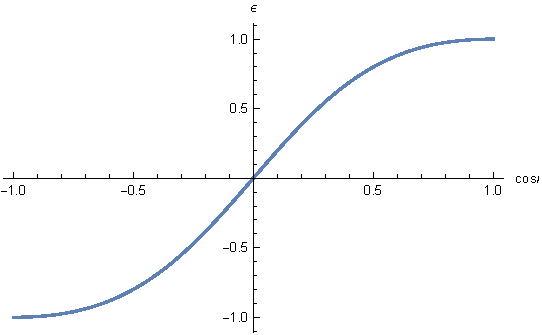
\includegraphics[width=\columnwidth]{ellip_cosi}
\caption{Ellipticity ($\epsilon$, ordinate) as a function of the cosine of the inclination ($\cos\iota$, abscissa) for the $\ell = |m| = 2$ GW strain from a nonprecessing compact binary inspiral, Eq.~\eqref{eq:ellip_cosi}. The signal from a face-on (face-off) binary has ellipticity $\epsilon = +1$ ($\epsilon=-1$), meaning it has a right-handed (left-handed) circular polarization.}
\label{fig:ellip_cosi}
\end{figure}

By comparison with Eq.~\eqref{eq:ellip_frame}, it is clear that Eq.~\eqref{eq:cbc} describe an elliptically polarized wave in a frame aligned with the polarization ellipse.
This is a consequence of the geometry of our assumed source, which is symmetric under reflections over the orbital plane: by choosing $\hat{y}$ to lie along the line of nodes, we also aligned our wave frame with the GW polarization ellipse.
Since our frame is already aligned  with the ellipse, we may just read off the ellipticity from Eq.~\eqref{eq:cbc} as
\beq \label{eq:ellip_cosi}
\epsilon = \frac{2 \cos\iota}{1 + \cos^2\iota}\, ,
\eeq
which is just the ratio of cross to plus amplitudes in this frame, and varies between $-1 \leq \epsilon \leq 1$ as required (Fig.~\ref{fig:ellip_cosi}).
This fact reveals that our decision to tie the polarization frame to the line of nodes was a good one: because this choice of wave-frame orientation preserves the symmetries of the source, it also happens to be aligned with the principal directions of the polarization ellipse.

Having specified $h_+$ and $h_\times$ in the standard source-based frame of Eq.~\eqref{eq:ellip_frame}, we need to determine how that frame itself is oriented with respect to the detectors in order to evaluate \eq{h}.
This is most easily done by expressing the components of $h_{ij}$ and $D_{ij}$ in a common basis, usually equatorial celestial coordinates for ground-based detectors.
If we use the standard convention for compact binaries described above (i.e., $\hat{y}$ along the line of nodes), then $\psi = 0$ must mean that the line of nodes points towards the celestial South \cite{LALSuite:source} (equivalently, the projection of orbital angular momentum is parallel to the celestial equator), see  Fig.~\ref{fig:waveframe}.
Knowing this, we can obtain expressions for $h_+$ and $h_\times$ in the celestial frame by measuring the angle from the line of ascending nodes to the celestial south and using \eq{htransf} with $\Delta\psi = \psi - 0 =\psi$.

In this convention, $\psi$ is identical to the \emph{position angle} of the source's orbital angular momentum $\Psi$; more generally, $\Psi = \psi \red{+} \Omega \red{-} \pi/2$ in terms of the longitude of the ascending node $\Omega$ with $\hat{x}$ as the origin of longitude ($\Omega = \pi/2$ in the default LIGO-Virgo convention) \cite{LALSuite:source}.
In fact, for a nonprecessing binary, the three angles $\psi$, $\Psi$ and $\theta$ can all be subsumed by a single parameter (usually written $\psi$) simultaneously encoding the orientation of our polarization basis, the alignment of the source in the sky, and the principal axes of the GW polarization ellipse.
We can then think of this angle as a property of the source to be measured from our data, rather than an arbitrary parameter orienting our frame.
Although this equivocation vastly simplifies analysis, it is useful to keep in mind that the three angles are conceptually distinct.

\begin{figure}
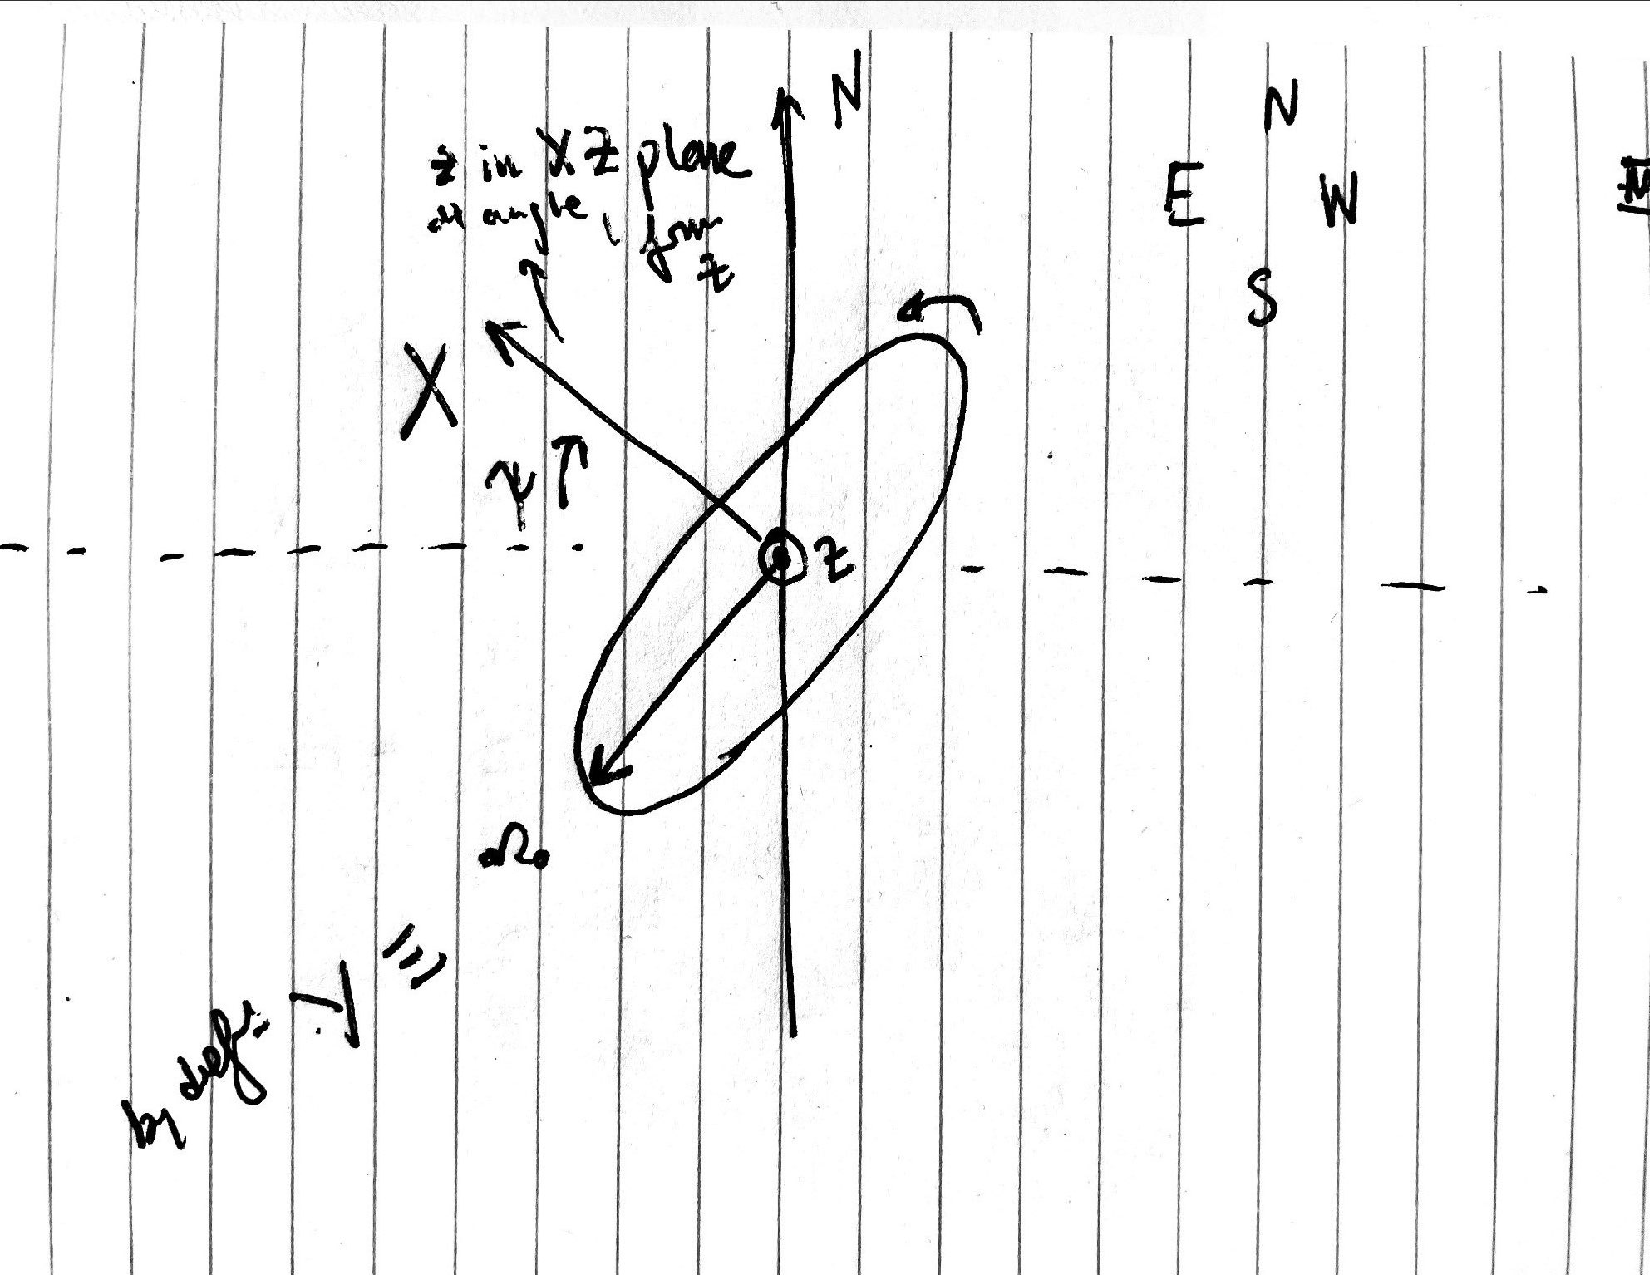
\includegraphics[width=\columnwidth]{waveframe}
\caption{Waveframe for a nonprecessing CBC source.}
\label{fig:waveframe}
\end{figure}


If the component spins are not (anti)aligned with the orbital angular momentum, the spins and the orbital plane will both precess.
As a consequence, the system will not be reflection symmetric and the GW signal will not be elliptically polarized overall.
In that case, it is still conventional to tie $\hat{x}$ to the source, referring to the line of nodes as oriented at some specific point in the binary evolution (e.g., when the detected GW signal reaches 20 Hz).

In summary, we can identify three conceptually distinct Cartesian frames: a wave frame that determines the principal directions along which we \emph{define} the effect of a plus vs cross wave; for an elliptical wave, an intrinsic polarization frame, representing the principal directions of the polarization ellipse; and a source frame, aligned with the symmetries of the source, or otherwise anchored to some defining feature of it; all of these can be specified in some astronomical frame, like ecliptic celestial coordinates.
For nonprecessing binaries, which are highly symmetric, we can define the source frame to make it always aligned with the polarization frame.

\subsection{Generic signals}

Although not all sources can be expected to be elliptically polarized, any signal can be modeled as a superposition of elliptically polarized components.
For example, that is the strategy taken by \textsc{BayesWave} \cite{Cornish:2014kda,Cornish:2020dwh}, which reconstructs generic GW signals by fitting a variable number of elliptically-polarized sine-Gaussians.%
\footnote{\textsc{BayesWave} can currently operate in two configurations: one which assumes the overall signal is elliptically polarized, and another which does not.}
It is also the case, in ringdown studies that fit the later portion of a compact binary signal as a superposition of elliptically polarized damped sinusoids \cite{Isi:2021iql}.

In analyses like these, it is not possible or useful to explicitly tie the polarization frame to properties of the source, since these analyses are not tailored to any specific source to begin with (or they purposely disregard source orientation information).
In that case, the model for $h_+$ and $h_\times$ can be defined in any arbitrary wave frame.
A common choice is to simply set $\psi = 0$ in the standard coordinates described in Sec.~\ref{sec:pol}, i.e., \red{with $\hat{y}$ pointing towards the celestial South} (Fig.~\ref{fig:waveframe}).
Having done so, all information regarding polarization orientation will be encoded in the $\theta$ parameter of Fig.~\ref{fig:ellipse}, with one value per elliptical mode in the decomposition.

Generalizing Eq.~\eqref{eq:ellip}, the decomposition of a signal into an elliptical basis will look like
\begin{subequations} \label{eq:ellip_sum}
\begin{equation} \label{eq:ellip_sum_p}
h_+ = \sum A_i(t) \left[\cos \Phi_i(t) \cos \theta_i - \epsilon_i \sin \Phi_i(t) \sin\theta_i \right] ,
\end{equation}
\begin{equation} \label{eq:ellip_sum_c}
h_\times = \sum A_i(t) \left[ \cos \Phi_i(t) \sin \theta_i + \epsilon_i \sin \Phi_i(t) \cos\theta_i \right] ,
\end{equation}
\end{subequations}
with $i$ indexing the elliptically polarized components.
The $A_i(t)$ and $\Phi_i(t)$ control the evolution of the polarization ellipses over time, including initial amplitude and phase $A_i \equiv A_i(t=0)$ and $\phi_i \equiv \Phi_i(t=0)$.
For example, in the case of ringdown templates, $A_i(t) = A_i \exp(-\gamma_i t)$ and $\Phi_i(t) = \omega_i t + \phi_i$ for some set of complex-valued frequencies $\tilde{\omega}_i = \omega_i - i\gamma_i$ to be inferred from the data together with polarization parameters $\{ A_i, \epsilon_i, \theta_i, \phi_i\}$.

In both cases, the elliptical decomposition is convenient because we do not expect the spectral content of the two polarizations to be totally independent.
This is true because (1) the same physical processes that generate plus also generate cross, and (2) even if, in principle, there could exist a source for which plus and cross were totally morphologically independent in \emph{some} frame (i.e., for some unknown choice of $\psi$ specific to each source) the plus and cross polarizations measured by generic observers would be linear combinations of the two independent components and, therefore, would look spectrally similar.

\section{Nontensor polarizations}

\newcommand{\xsym}{\ensuremath{\rm x}}
\newcommand{\ysym}{{\rm y}}
\newcommand{\bsym}{{\rm b}}
\newcommand{\lsym}{{\rm l}}
\newcommand{\hx}{h_{\xsym}}
\newcommand{\hy}{h_{\ysym}}
\newcommand{\hb}{h_{\bsym}}
\newcommand{\hlon}{h_{\lsym}}

Metric theories beyond GR may allow up to six independent polarizations, including the two tensor $+$ and $\times$ modes expected in GR.
The discussion above generalizes easily to include those additional modes, starting with an enhanced version of the driving matrix in Eq.~\eqref{eq:hij},
\beq \label{eq:hij_ngr}
(h_{ij}) = \begin{pmatrix}
\hb + h_+ & h_\times  & \hx  \\
h_\times  & \hb - h_+ & \hy  \\
\hx    & \hy    & \hlon
\end{pmatrix} ,
\eeq
where, in addition to plus and cross, also appear the vector-$x$ (\xsym) and vector-$y$ modes (\ysym), as well as the scalar breathing (\bsym) and longitudinal (\lsym) modes.%
\footnote{There are other possible normalizations in use in the literature, e.g., $\hlon \to \sqrt{2} \hlon$.}
Equivalently, as above, we can write this as a weighted sum over polarization tensors,
\beq
h_{ij} = \sum_p h_p\, e^p_{ij} \, ,
\eeq
for $p$ in $\{+,\times, \xsym, \ysym, \bsym, \lsym\}$, and polarization tensors $e^p_{ij}$ defined implicitly by comparison with Eq.~\eqref{eq:hij_ngr}.
Generally, the $h_p$ are functions of time, as for plus and cross above.

The considerations presented above regarding wave frame orientation and antenna pattern symmetries apply just as well to the generalized polarization tensor of Eq.~\eqref{eq:hij_ngr}, except for the different properties that the beyond-GR modes exhibit under rotations.
A rotation by $\Delta \psi$ around the line of propagation transforms the two vector amplitudes by
\begin{subequations} \label{eq:htransf_v}
\beq
\hx \rightarrow \hx' = \hx \cos \Delta \psi - \hy \sin \Delta\psi \, ,
\eeq
\beq
\hy \rightarrow \hy' = \hx \cos \Delta \psi + \hy \sin \Delta\psi \, ,
\eeq
\end{subequations}
reflecting the fact that these are the components of a spin-weight $s=1$ field (hence ``vector'').
On the other hand, the two scalar modes are invariant under rotations around $z$,
\begin{subequations} \label{eq:htransf_s}
\beq
\hb \rightarrow \hb' = \hb\, ,
\eeq
\beq
\hlon \rightarrow \hlon' = \hlon\, ,
\eeq
\end{subequations}
revealing that these behave as spin-weight $s=0$ fields (hence ``scalar'').

With similar assumptions as in the GR case, the detector output can be written as a sum over polarizations weighted by antenna patterns,
\beq \label{eq:h_ngr}
h(t) = \sum_p F_p(\alpha, \delta; \psi)\, h_p(t)\, ,
\eeq
with $F_p \equiv D^{ij} e^p_{ij}$ as before. 

As it turns out, differential-arm GW detectors are only sensitive to the traceless linear combination of the two scalar polarizations.
In terms of the breathing and longitudinal modes above, this is
\beq
h_{\rm s} \equiv \hb - 2\hlon\, ,
\eeq
which is the only scalar mode measurable by existing detectors.
Equivalently, the antenna patterns for the breathing and longitudinal modes are the same up to an overall constant (with our normalization, $F_{\bsym} = -F_{\lsym}$).
Therefore, the two terms are degenerate in Eq.~\eqref{eq:h_ngr} and their contributions cannot be disentangled in a model-independent way, i.e., without theory- and source-specific information about the specific morphology of the $\hb(t)$ and $\hlon(t)$ functions.
For unmodeled analyses, it thus suffices to include only one scalar term in Eq.~\eqref{eq:h_ngr}---commonly that for the breathing mode---so that the sum is over only five polarizations instead of six.

\section{Conclusion}

\begin{acknowledgments}
% NASA
M.I.\ is supported by NASA through the NASA Hubble Fellowship
grant No.\ HST-HF2-51410.001-A awarded by the Space Telescope
Science Institute, which is operated by the Association of Universities
for Research in Astronomy, Inc., for NASA, under contract NAS5-26555.
% % LIGO
% M.I.\ is a member of the LIGO Laboratory.
% LIGO was constructed by the California Institute of Technology and
% Massachusetts Institute of Technology with funding from the National
% Science Foundation and operates under cooperative agreement PHY-0757058.
% DCC
This paper carries LIGO document number \dcc{}.
\end{acknowledgments}

\bibliography{refs}

\end{document}
%
% ****** End of file apstemplate.tex ******
